\section{Introduction}

This report covers all three parts of the project. In the work with the later parts of the project, the components of the earlier parts have been changed to accommodate altered needs.\\
The First problem consisted of expanding the implementation of rdt in the given project, from reliable transfer between two stations, to reliable transfer from each station with one or more neighbouring stations.\\
The second part consisted of designing and implementing a datagram network layer for routing datagrams in the network.\\
The final part consisted of implementing a connection-oriented transport layer and showing how an application in the application layer utilizes the network stack.\\

Figure \ref{fig:GivenTopology} from the project description illustrates the constellation of stations and their types in the network layout used for testing.Note that the routers are called 1 and 2 rather than C and D, both in the source code and this report, to ease distinction between routers and hosts.
\begin{figure}[H]
\centering
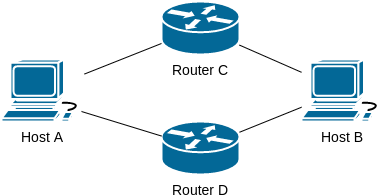
\includegraphics[width=0.5\textwidth]{../figs/network-topology.png}
\caption{Topology for which it is required that the implementation functions}
\label{fig:GivenTopology}
\end{figure}


\subsection{Terms}
The following are additional terms used as shorthands:
\begin{itemize}
\item LL: Link Layer
\item NL: Network Layer
\item TL: Transport Layer
\item AL: Application Layer, sometimes implicitly the application in the application layer.
\end{itemize}
